\section{Nutrient-Mediated Growth Rate Control Dictates both Ribosomal Content and Cell Size}
\label{sec:minimal_model}
While the preceding section highlights a dominant role for ribosomes in setting
the achievable growth rate, our analysis thus far has also shown how the
proteomic content and cell size will need to change in response to variable
growth conditions and growth rate. The specific mechanism of growth rate control
under nutrient limitation that leads to the observed exponential scaling in cell
size in \textit{E. coli} and other bacteria, however, has remained unclear
\citep{si2017, harris2018, ojkic2019}. Here we consider the consequences of the
translation-limiting growth rate on cell size and its underlying mechanism.

Under translation-limited growth conditions (> $\approx$ 0.5 hr$^{-1}$), cells can
only increase growth rate by increasing ribosome content. While the simple
addition of more ribosomes is likely constrained by macromolecular crowding
\citep{delarue2018, solerbistue2020}, cells appear to bias their protein
synthesis specifically in favor of ribosomes as they increase their size. To see
this, we have calculated the position-dependent protein expression across the
chromosome by a running Gaussian average of protein copy number (20 kbp st. dev.
averaging window) based on each gene's transcriptional start site
[\FIG{elongation_rate_model}(A)]. These were median-subtracted to account  for
the increasing total protein abundance with $\langle$\# ori$\rangle$. In
particular, we find that the deviations in protein expression with $\langle$\#
ori$\rangle$ are largely restricted to regions of ribosomal protein genes. This
result suggests that $\Phi_R$ is also being tuned in proportion to $\langle$\#
ori$\rangle$ under nutrient-limited growth. Importantly, it is through this
additional dependence on $\Phi_R$, combined with the exponential increase in
$\langle$\# ori$\rangle$ that was noted in the previous section, that \textit{E.
coli} exhibits an exponential increase in cell size with growth rate at moderate to
fast growth rates.

In \textit{E. coli}, an accumulation of de-acylated tRNAs at the ribosome's
A-site leads to a strong increase in (p)ppGpp synthesis activity by the enzyme
RelA \citep{hauryliuk2015}. While conventionally associated with a dynamic
global response to changes in nutrient conditions through the stringent
response, (p)ppGpp increasingly appears to play a role in both the control of
the active ribosomal fraction and cell size homeostasis under steady-state
nutrient-limited growth \citep{dai2016, zhu2019, Buke2020, vadia2017,
parker2020}. It is now well-documented that \textit{E. coli} cells add a
constant volume per origin of replication, which is robust to a remarkable array
of cellular perturbations \citep{si2017}. Here, there is increasing evidence
that (p)ppGpp acts to inhibit the initiation of DNA replication
\citep{fernandezcoll2020}, providing a potential mechanism for cells to lower
$\langle$\# ori$\rangle$ and maintain a smaller, more economical cell size in
poorer nutrient conditions. From the proteomic measurements, we find that cells
also vary their ribosome copy number in direct proportion to $\langle$\#
ori$\rangle$ [\FIG{elongation_rate_model}(B)]. With cellular (p)ppGpp levels
following directly from the state of ribosomal activity, cells appear to use
ribosome activity as a direct proxy for nutrient availability, and hence are
able to better match cell size (and $\langle$\# ori$\rangle$) and ribosomal
content according to the required biosynthetic capacity for growth
[\FIG{elongation_rate_model}(C)].

To consider this quantitatively, we assume that cells modulate their proteome
(total number of peptide bonds $N_\text{pep}$, number of ribosomes $R$, and
ribosomal fraction $\Phi_R$) to better maximize their rate of peptide elongation
$r_t$. The elongation rate $r_t$ will depend on how quickly ribosomes can match
codons with an amino-acyl tRNA, along with the subsequent steps of peptide bond
formation and translocation. This ultimately depends on the cellular
concentration of amino acids, which we treat as a single effective species,
$[AA]_\text{eff}$ \citep{bosdriesz2015}. Having found that cells do not appear limited
in their synthesis of tRNA or GTP, we determine the rate of peptide elongation
$r_t$ and achievable growth rate as simply depending on the supply of amino
acids (and, therefore, also amino-acyl tRNAs), through a parameter $r_{AA}$ in
units of AA per second, and the rate of amino acid consumption by protein
synthesis ($r_t \times R \times f_a$). In \FIG{elongation_rate_model}(D), we
illustrate how the elongation rate will depend on the ribosomal copy number for
constant $r_{AA}$, and further described in the Supplemental Section
"Derivation of Minimal Model for Nutrient-Mediated Growth Rate Control".

% In \FIG{elongation_rate_model}(B), we illustrate how the elongation rate will
% depend on the ribosomal copy number. Here, we have considered an arbitrarily
% chosen $r_{AA} = 5\times 10^6$ AA $\cdot$ s$^{-1} \cdot$ \textmu m$^{-3}$ and
% $f_a = 1$ for a unit cell volume $V = 1$fL (we provide the interactive figure
% \FIGSUPP[elongation_rate_model]{model_explorer} which allows the user to explore
% different regimes of this parameter space). At low ribosome copy numbers,
% the
% observed elongation rate is dependent primarily on $[AA]_\text{eff}$ through
% $r_{AA}$ [as $r_t^{\text{max}} \times R \times f_a << r_{AA}$, point (1) in
% \FIG{elongation_rate_model}(B)]. As the ribosome copy number is increased
% such that the amino acid supply rate and consumption rate are nearly equal
% [point (2) in \FIG{elongation_rate_model}(B)], the observed elongation rate
% begins to decrease sharply. When the ribosome copy number is increased even
% further, consumption at the maximum elongation rate exceeds the supply rate,
% yielding a significantly reduced elongation rate [point (3) in
% \FIG{elongation_rate_model}{B)]. While the elongation rate will always be
% dominated by the amino acid supply rate at sufficiently low ribosome copy
% numbers, the elongation rate at larger ribosome abundances can be increased
% by tuning $f_a$ such that not all ribosomes are elongating, reducing their
% total consumption rate.

\begin{figure}
    \centering{
    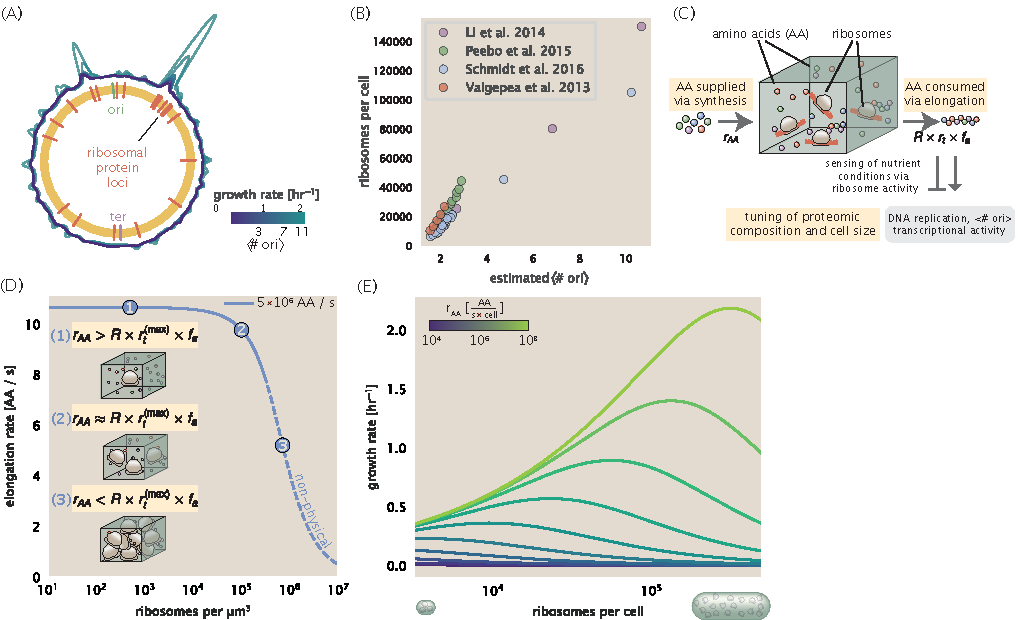
\includegraphics[width=0.8\textwidth]{main_figs/fig6_elongation_model_update.pdf}
    \caption{\textbf{Coordination of cell size and proteomic composition via ribosome activity.}
    (A) A running
        Gaussian average (20 kbp st. dev.) of protein copy number is calculated
        for each growth condition considered by \citep{schmidt2016} based
        on each gene's transcriptional start site. Since total
        protein abundance increases with growth rate, protein copy numbers are
        median-subtracted to allow comparison between growth conditions.
        $\langle$\# ori$\rangle$ are estimated using the data in (A) and
        Equation \ref{eq:Nori}.
    (B) Plot of the ribosome copy number estimated from the
        proteomic data against the estimated $\langle$\# ori$\rangle$ (see Supplemental
        Section "Estimation of $\langle$\# ori$\rangle$/ $\langle$\# ter$\rangle$ and $\langle$\# ori$\rangle$ for additional details).
    (C) We consider a unit volume of cellular material
        composed of amino acids (colored spheres) provided at a supply rate
        $r_{AA}$. These amino acids are polymerized by a pool of ribosomes
        (brown blobs) at a rate $r_t \times R \times f_a$, where $r_t$ is the
        elongation rate, $R$ is the ribosome copy number in the unit volume, and
        $f_a$ is the fraction of those ribosomes actively translating. In addition to
        determining total protein synthesis rate, the nutrient status is gauged
        by any accumulation of de-acylated tRNAs and synthesis of the secondary messenger
        (p)ppGpp, which ultimately determine $\langle$\# ori$\rangle$, cell size,
        and proteomic composition.
    (D) The observed elongation rate is plotted as a function of the number of ribosomes.
        The three points correspond to three regimes of ribosome copy numbers
        and are shown schematically on the left-hand side. The region of the
        curve shown as dashed lines represents a non-physical copy number, but
        is shown for illustrative purposes. This curve was generated using an
        amino acid supply rate of $5 \times 10^6$ AA / s, a maximal elongation
        rate of 17.1 AA / s, $f_a = 1$, and a unit cell volume of 1 fL.
        See Supplemental Section "Derivation of Minimal Model for Nutrient-Mediated
        Growth Rate Control" for additional model details. (C) The cellular
        growth rate is plotted as a function of total cellular ribosome copy
        number for different cellular amino acid supply rates, with blue and
        green curves corresponding to low and high supply rates, respectively.
        As the ribosome copy number is increased, so too is the cell size and
        total protein abundance $N_\text{pep}$.
    }
    \label{fig:elongation_rate_model}
    }
\end{figure}

To relate elongation rate to growth rate, we constrain the set of parameters
based on our available proteomic measurements; namely, we restrict the values of
$R$, $N_{pep}$, and cell size to those associated with the amalgamated proteomic
data (described in the Supplemental Section "Estimation of Total Protein Content per
Cell"). We then consider how changes in the nutrient conditions, through the
parameter $r_{AA}$, influence the maximum growth rate as determined by
\EQ{lam_limited}. \FIG{elongation_rate_model}(E) shows how the growth rate
depends on the rate of amino acid supply $r_{AA}$ as a function of the cellular
ribosome copy number. A feature immediately apparent is the presence of a
maximal growth rate increases with increasing $r_{AA}$. Importantly, however,
there is an optimum set of $R$, $N_\text{pep}$, and cell size that are strictly
dependent on the value of $r_{AA}$. This shows that increasing the ribosomal
concentration beyond the cell's metabolic capacity will have the adverse
consequence of depleting the supply of amino acids and lead to a concomitant
decrease in the elongation rate $r_t$ [\FIG{elongation_rate_model}(D)] and
growth rate. This helps us understand that while it is important for cells to
increase their ribosomal content and total protein content (and hence, also cell
size) in order to increase growth rate, cells will better maximize their
achievable growth rate by tuning these parameters according to the available
nutrient conditions, since this is ultimately what allows cells to reach the
peak for each curve shown in \FIG{elongation_rate_model}(E).

Also of note is the growth rate trends observed at low values of $r_{AA}$
[purple and blue lines in \FIG{elongation_rate_model}(E)], representative of
growth in nutrient-poor media. In these conditions, there no longer exists a
peak in the maximum growth rate, at least within the range of
physiologically-relevant ribosome copy numbers considered here. This is the
regime, associated with slower growth rates, where cells limit their pool of
actively translating ribosomes by decreasing $f_a$ (\FIG{ribosome_limit}(A),
inset), likely due to having excess ribosomes relative to the cell's metabolic
capacity. By reducing the fraction of actively translating ribosomes, we find
that cells instead appear to be prioritizing their pool of available amino acids
$[AA]_\text{eff}$ in order to increase their translation elongation rate.
Consistent with this hypothesis and our model, while inhibition of translation
with chloramphenicol further reduces the fraction of actively translating
ribosomes $f_a$, it results in an increase in the elongation rate
\citep{dai2016}.
